\documentclass[a4paper]{article}
%Fonts 
\fontencoding{T1}
\usepackage{textcomp}
\usepackage{microtype}
\usepackage{mathpazo}
%\usepackage[oldstyle]{libertine}
%%\usepackage{libertinust1math}
%\usepackage[scaled=0.81]{beramono}


\usepackage{amsmath}
\usepackage{graphicx}
\usepackage{upquote}
\usepackage{listings}
\usepackage{xcolor}
\usepackage{siunitx}
\usepackage{hyperref}
\usepackage{natbib}

\usepackage{parskip}
\setlength{\parindent}{0pt}
\DeclareSIUnit{\year}{y}
\usepackage{xsim}
\loadxsimstyle{layouts}

\loadxsimstyle{layouts}

\DeclareExerciseHeadingTemplate{custom}
  {\section{\XSIMexpandcode{\XSIMtranslate{default-heading}}}}

\DeclareExerciseEnvironmentTemplate{custom}
  {%
    \IfInsideSolutionTF
      {\label{sol:\ExerciseID}}
      {\label{ex:\ExerciseID}}
      \par
    \noindent\llap{%
      \footnotesize\sffamily
      \IfInsideSolutionTF
        {%
          \XSIMmixedcase{\GetExerciseParameter{exercise-name}}
          on \hyperref[ex:\ExerciseID]{page~}\pageref{ex:\ExerciseID}.%
        }
        {%
          \XSIMmixedcase{\GetExerciseParameter{solution-name}}
          on \hyperref[sol:\ExerciseID]{page~}\pageref{sol:\ExerciseID}.%
        }%
      \hspace*{\marginparsep}%
    }%
    \textbf
      {%
        \XSIMmixedcase{\GetExerciseName}%
        \IfInsideSolutionTF
          {
            to \hyperref[ex:\ExerciseID]{\GetExerciseParameter{exercise-name}%
            ~\GetExerciseProperty{counter}}\\%%
          }
          {%
            ~\GetExerciseProperty{counter}
            \GetExercisePropertyT{subtitle}
              { {\normalfont\itshape\PropertyValue}}%
          }%
      }
  }
  {\par}
\xsimsetup{
  exercise/template = custom ,
  solution/template = custom ,
  print-solutions/headings-template = custom
}

\title{River flow and morpholgy -- PC practical 2}
\author{B. Vermeulen}
%\qformat{\textbf{Exercise \thequestion} \hfill}

\newcommand{\der}[2]{\dfrac{\mathrm{d}#1}{\mathrm{d}#2}}
\newcommand{\pder}[2]{\dfrac{\partial#1}{\partial#2}}
\newcommand{\lpder}[2]{\partial#1/\partial#2}
\newcommand{\pdder}[2]{\dfrac{\partial^2#1}{\partial#2^2}}

\definecolor{codegreen}{rgb}{0,0.6,0}
\definecolor{codegray}{rgb}{0.5,0.5,0.5}
\definecolor{codepurple}{rgb}{0.58,0,0.82}
\definecolor{backcolour}{rgb}{0.95,0.95,0.92}

\lstdefinestyle{mystyle}{
    backgroundcolor=\color{backcolour},
    commentstyle=\color{codegreen},
    keywordstyle=\color{blue},
    numberstyle=\tiny\color{codegray},
    stringstyle=\color{codepurple},
    basicstyle=\ttfamily\footnotesize,
    breakatwhitespace=false,
    breaklines=true,
    captionpos=b,
    keepspaces=true,
    numbers=left,
    numbersep=5pt,
    showspaces=false,
    showstringspaces=false,
    showtabs=false,
    tabsize=2,
}

\lstset{
  style=mystyle, 
  language=Matlab,
  deletekeywords={ans, xlabel, ylabel, plot, legend, title, close, all},
  morekeywords={*, classdef, properties, methods}
}

% hyperref settings
\colorlet{link}{black!60!red}
%\colorlet{link}{black}
\hypersetup{
    unicode=false,          % non-Latin characters in Acrobat's bookmarks
    pdftoolbar=true,        % show Acrobat's toolbar?
    pdfmenubar=true,        % show Acrobat's menu?
    pdffitwindow=false,     % window fit to page when opened
    pdfstartview={FitH},    % fits the width of the page to the window
    pdftitle={River flow and morphology},    % title
    pdfauthor={HWM},     % author
    pdfcreator={HWM},   % creator of the document
    pdfproducer={HWM}, % producer of the document
    pdfnewwindow=true,      % links in new PDF window
    colorlinks=true,       % false: boxed links; true: colored links
    linkcolor=link,          % color of internal links (change box color with linkbordercolor)
    citecolor=link,        % color of links to bibliography
    filecolor=link,      % color of file links
    urlcolor=link,           % color of external links
}

\begin{document}
\maketitle
\tableofcontents


\section{Introduction}
\label{sec:intro}
This practical is part of the course ``River flow and morphology''. This practical covers topics concerning the morphological development of rivers. At the end of this practical student are expected to be able to:
\begin{enumerate}
  \item Explain the initial morphological response of a river to non-uniform steady flow
  \item Interpret results concerning the long term morphological development of a river after a change in forcings or geometry.
  \item Evaluate morphodynamic development in terms of advective and diffusive behaviour
  \item Relate the advective and diffusive morphodynamic behaviour to the scale of a disturbance
\end{enumerate}

In the first part of the practical the backwater example in the lecture is reproduced in MATLAB and the initial morphological response and the long term morphology are studied.
Afterwards, a new case is introduced that will be studied in a similar way as the example from the lecture notes.
Eventually a model is used to study the morphodynamic behaviour of small and large scale bed perturbations.

\section{Initial erosion and sedimentation}

\subsection{River widening}
First of all, make sure you download the updated \lstinline{Backwater.m} file from Brightspace, for the second pc practical.

We will continue working on the example of the river widening. During the first practical we already created three \lstinline{Backwater} objects to simulate the non-uniform flow in the river. We ended up with the following code (also available on Brightspace under ``Pc practical 1'' in the file \lstinline{lecture_notes_example.m}):
\lstinputlisting{matlab/lecture_notes_hydrodynamics.m}
Running this script will produce \autoref{fig:hydrodynamics_widening}.
\begin{figure}[h]
  \centering
  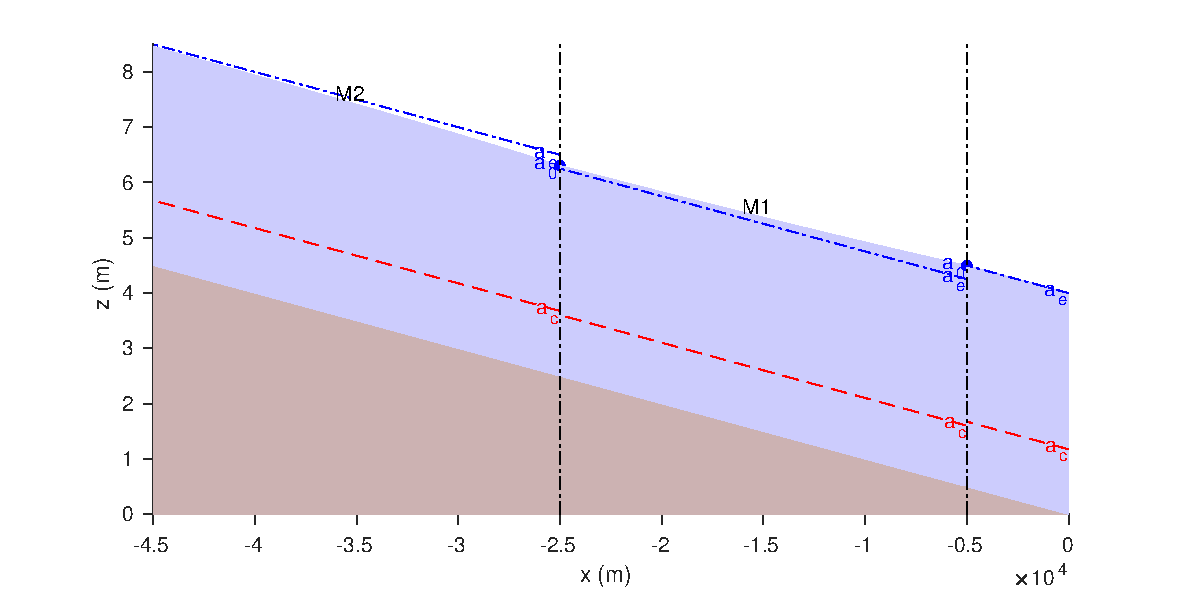
\includegraphics[width=\linewidth]{matlab/backwater_lecture_notes.pdf}
  \caption{Hydrodynamic situation for river widening}
  \label{fig:hydrodynamics_widening}
\end{figure}

Now, we want to asses how the river will initially respond to this widening. We do this based on Exner's equation:
\begin{align*}
  (1-\epsilon)\pder{z_b}{t}+\pder{q_s}{x}=0
\end{align*}
This means that $\lpder{z_b}{t}\propto-\lpder{q_s}{x}$. Since $q_s\propto u$ we can also infer that $\lpder{z_b}{t}\propto-\lpder{u}{x}$.
So we will first make a plot of how velocity varies along the reach:
\begin{lstlisting}
R.plot_velocity()
\end{lstlisting}
This produces \autoref{fig:velocity_widening} 
\begin{figure}[ht]
  \centering
  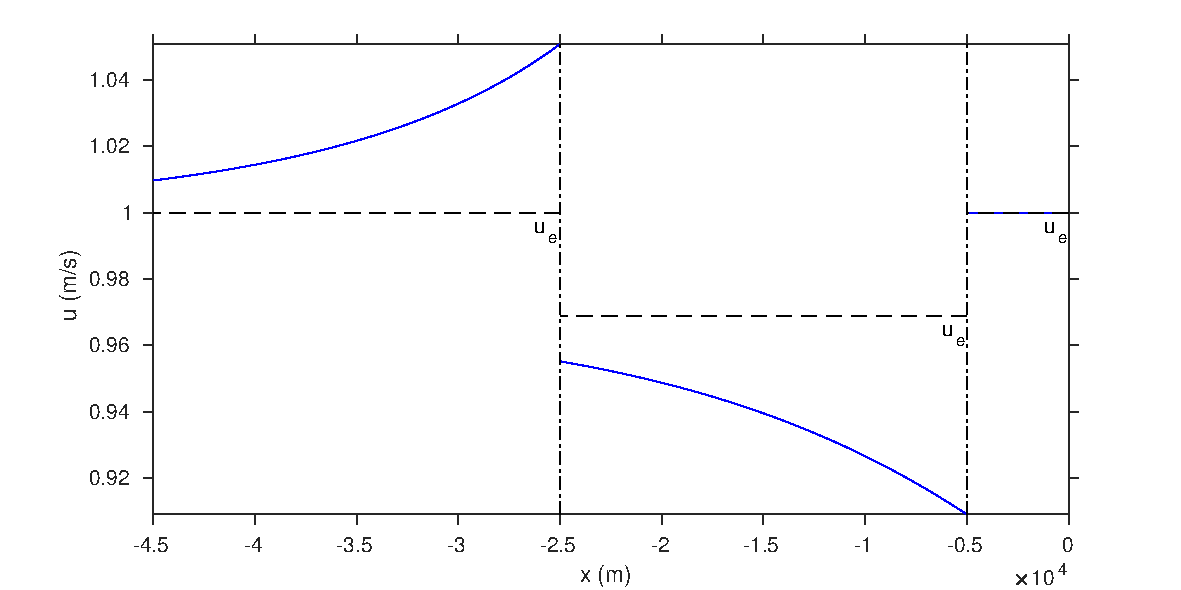
\includegraphics[width=\linewidth]{matlab/velocity_widening.pdf}
  \caption{Variation of velocity along the backwaters (blue line).}
  \label{fig:velocity_widening}
\end{figure}
\begin{exercise}
  Explain what the dashed lines mean and also provide an explanation for the variation of the velocity (blue line).
\end{exercise}
\begin{solution}
  The dashed lines indicate the equilibrium velocity. From equation 4.2 in the lecture notes we can see that a river widening results in a lower equilibrium depth. This, in turn results in a lower equilibrium velocity (law of Chezy). So we see that the equilibrium velocity in the widened reach is low than the equilibrium velocity in the upstream and downstream reach. 

  The velocity profile can now be understood with respect to the equilibrium line. If the depth would be equal to the equilibrium depth (dash dotted blue line in \autoref{fig:hydrodynamics_widening}) the velocity would be equal to the equilibrium velocity. Since in the upstream reach the depth is lower, the velocity must be larger, and increasing downstream. The opposite is true for the middle reach. Here, the depth is increasing and higher than the equilibrium depth, so the velocity will be lower than the equilibrium depth and decreasing. In the downstream reach the flow is in equilibrium.
\end{solution}

Now, from the velocity curves we can derive what the $\lpder{u}{x}$ curves will look like.
For this we run:
\begin{lstlisting}
R.plot_vel_gradient()
\end{lstlisting}
This produces \autoref{fig:velgrad_widening}.
\begin{figure}[ht]
  \centering
  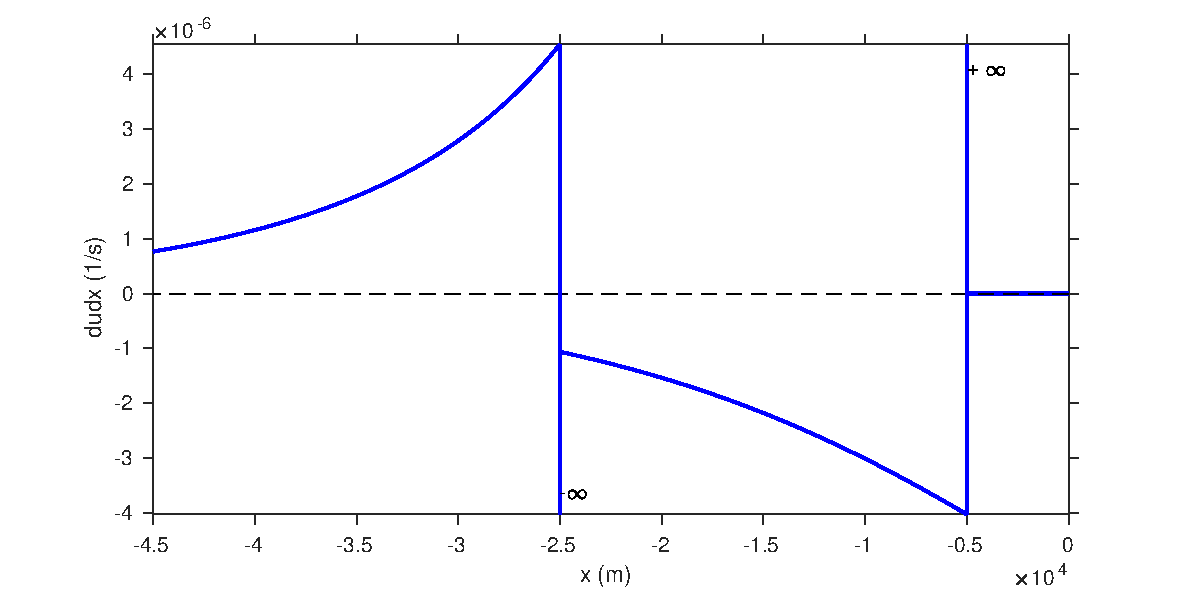
\includegraphics[width=\linewidth]{matlab/velgrad_widening.pdf}
  \caption{Downstream gradient of velocity.}
  \label{fig:velgrad_widening}
\end{figure}
\begin{exercise}
  Explain the variation of the velocity gradient in \autoref{fig:velgrad_widening}. What do those vertical lines mean in the graph?
\end{exercise}

\begin{solution}
  First thing to notice is the dashed line indicating a gradient of zero (i.e. the velocity does not change along the distance of the river). In the upstream reach the velocity is increasing, which means that we have a positive slope. The curve for the velocity is curving upward and we know from theory that it will follow a nearly exponential shape. This means that also the derivative will follow an exponential shape (since the derivative of an exponential is again an exponential).
  
  At the interface between the upstream and middle reach, the velocity suddenly drops due to the widening. A vertical drop in velocity corresponds to a $-\infty$ slope, which is represented by the vertical line in the gradient plot. After the drop at the interface we have an exponential drop in velocity in the middle section. This is reflected in the gradient graph by a negative exponential value. 
  
  At the interface between the middle and downstream reach, the velocity suddenly increases, which is reflected by a line going to $+\infty$ in the gradient plot. In the downstream reach te flow is in equilibrium, which means that the velocity does not change along the river, so the gradient is zero.
\end{solution}

Now we can make a similar figure for the gradient in sediment transport. The \lstinline{Backwater} class, uses a simplified sediment transport formula:
\begin{align*}
  q_s=mu^n
\end{align*}
\begin{exercise}
  What are the units of the constant \lstinline{m}?
\end{exercise}

\begin{solution}
  The units of \lstinline{m} are found as:
  \begin{align*}
      &q_s=mu^n \Rightarrow [q_s]=[m][u]^n \Rightarrow [m]=\dfrac{[q_s]}{[u]^n} \Rightarrow [m]=\dfrac{\si{\m\squared\per\s}}{(\si{\m\per\s})^n}\Rightarrow\\
      &[m]=\si{m\tothe{2-n}\s\tothe{n-1}}
  \end{align*}
\end{solution}

You can see the sediment transport constants in the \lstinline{Backwater} objects:
\begin{lstlisting}
>> R(1).m_sed_transp

ans =

   2.3000e-04

>> R(2).n_sed_transp

ans =

     5

>> 
\end{lstlisting}

Now we can plot the downstream gradient of sediment transport:

\begin{lstlisting}
R.plot_qs_gradient()
\end{lstlisting}

This produces \autoref{fig:qsgrad_widening}

\begin{figure}[ht]
  \centering
  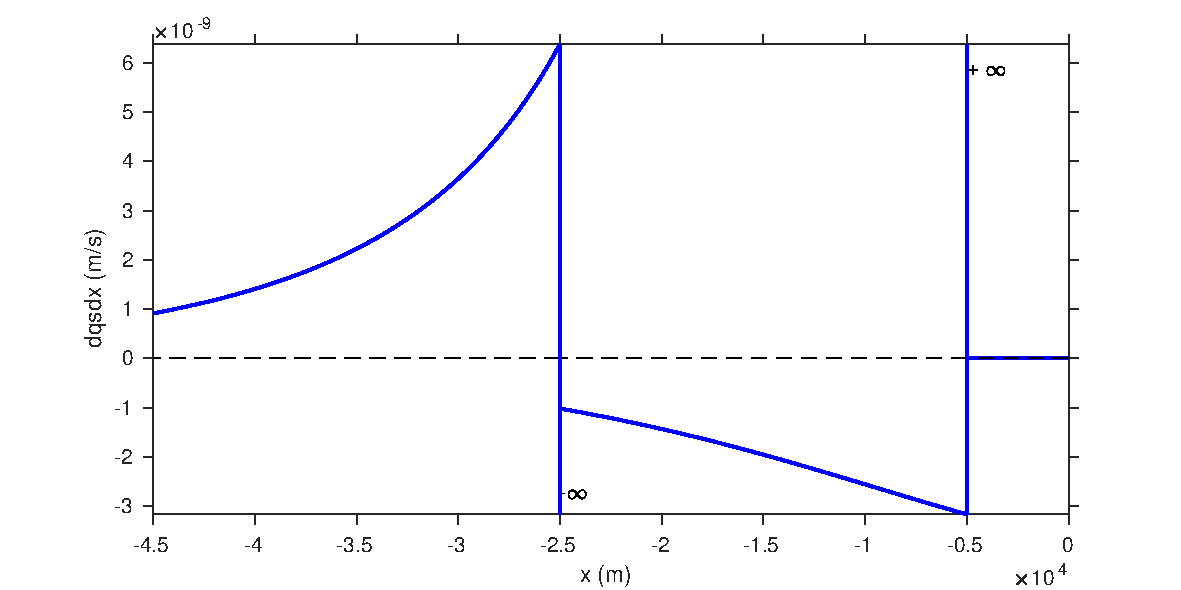
\includegraphics[width=\linewidth]{matlab/qsgrad_widening.pdf}
  \caption{Downstream gradient of sediment transport.}
  \label{fig:qsgrad_widening}
\end{figure}

To little surprise, the gradient in sediment transport is very similar to the gradient in velocity.

Eventually we can plot the temporal change in the bed, i.e. the erosion or sedimentation rate:

\begin{lstlisting}
R.plot_zb_gradient()
\end{lstlisting}

\begin{figure}[ht]
  \centering
  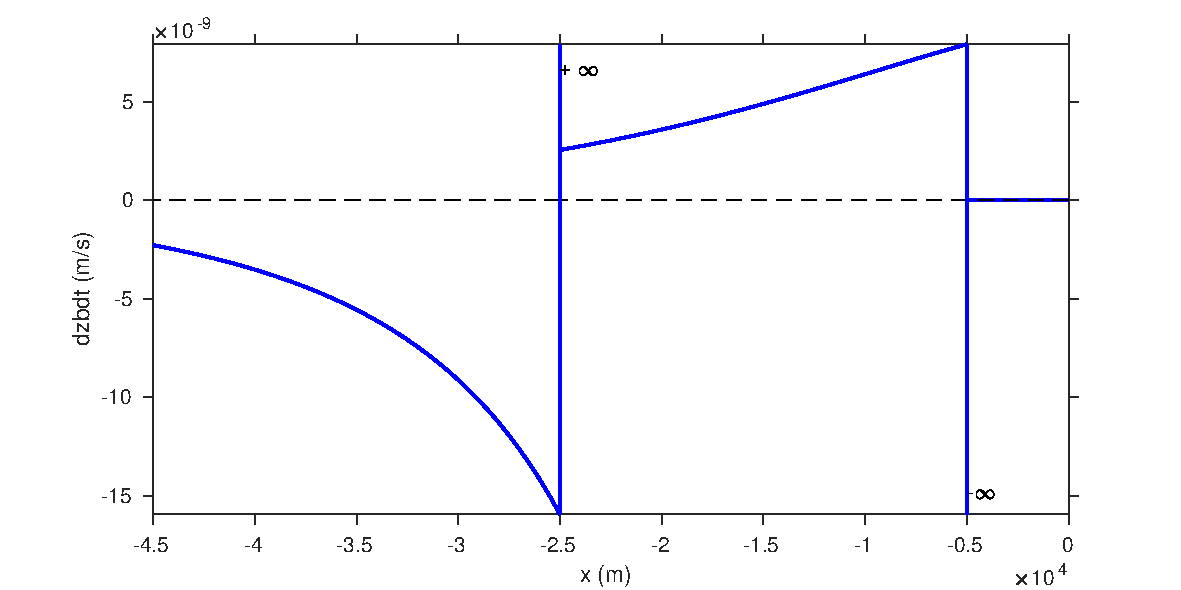
\includegraphics[width=\linewidth]{matlab/zbgrad_widening.pdf}
  \caption{Initial erosion and sedimentation rates.}
  \label{fig:zbgrad_widening}
\end{figure}

\begin{exercise}
  Explain the erosion and sedimentation rates. What happens at the $+\infty$ and $-\infty$ lines?
\end{exercise}

\begin{solution}
  In the upstream reach, we have a drawdown and as a result velocity increases in downstream direction. This results in a downstream increasing sediment transport. The additional sediment that is transported comes for the eroding bed. In the middle reach we have a backwater effect with depth increasing and velocity decreasing in downstream direction. As a result sedimentation occurs.
  
  At the $+\infty$ we have a sudden decrease in velocity due to the widening. This results in a very strong deposition. A depositional front develops that travels downstream. The height of this front will be such that the it exactly compensates the river widening, with an equal velocity just upstream and just downstream of the widening.
  
  A similar thing happens at the downstream end of the widening, but here we have a sudden acceleration, with an erosional front as a result. This erosional front will propagate downstream.
\end{solution}

\begin{exercise}
  The rates are really small O(-9). Does this make sense?
\end{exercise}

\begin{solution}
  The rates in the equation are given in \si{\m\per\s}. An erosion rate of \SI{15e-9}{\m\per\s} corresponds to an erosion rate of:
  \begin{align*}
      \dfrac{\mathrm{d} z_b}{\mathrm{d} t}=\SI{-15e-9}{\m\per\s}=&\SI{-15e-9}{\m\per\s}\cdot\SI{3600}{\s\per\hour}\cdot\SI{24}{\hour\per\day}\cdot\SI{365}{\day\per\year}=\\
      =&\SI{-0.473}{\m\per\year}
  \end{align*}
  This is a reasonable erosion rate.
\end{solution}
Since we often want to plot these graphs together there is a plot function that will do this for us:
\begin{lstlisting}
R.plot_initial_ersed()
\end{lstlisting}
This produces \autoref{fig:initersed_widening}. In this figure the $x$ axes of the graphs are linked, so zooming in on one graph, will also zoom in on the others.
\begin{figure}[ht]
  \centering
  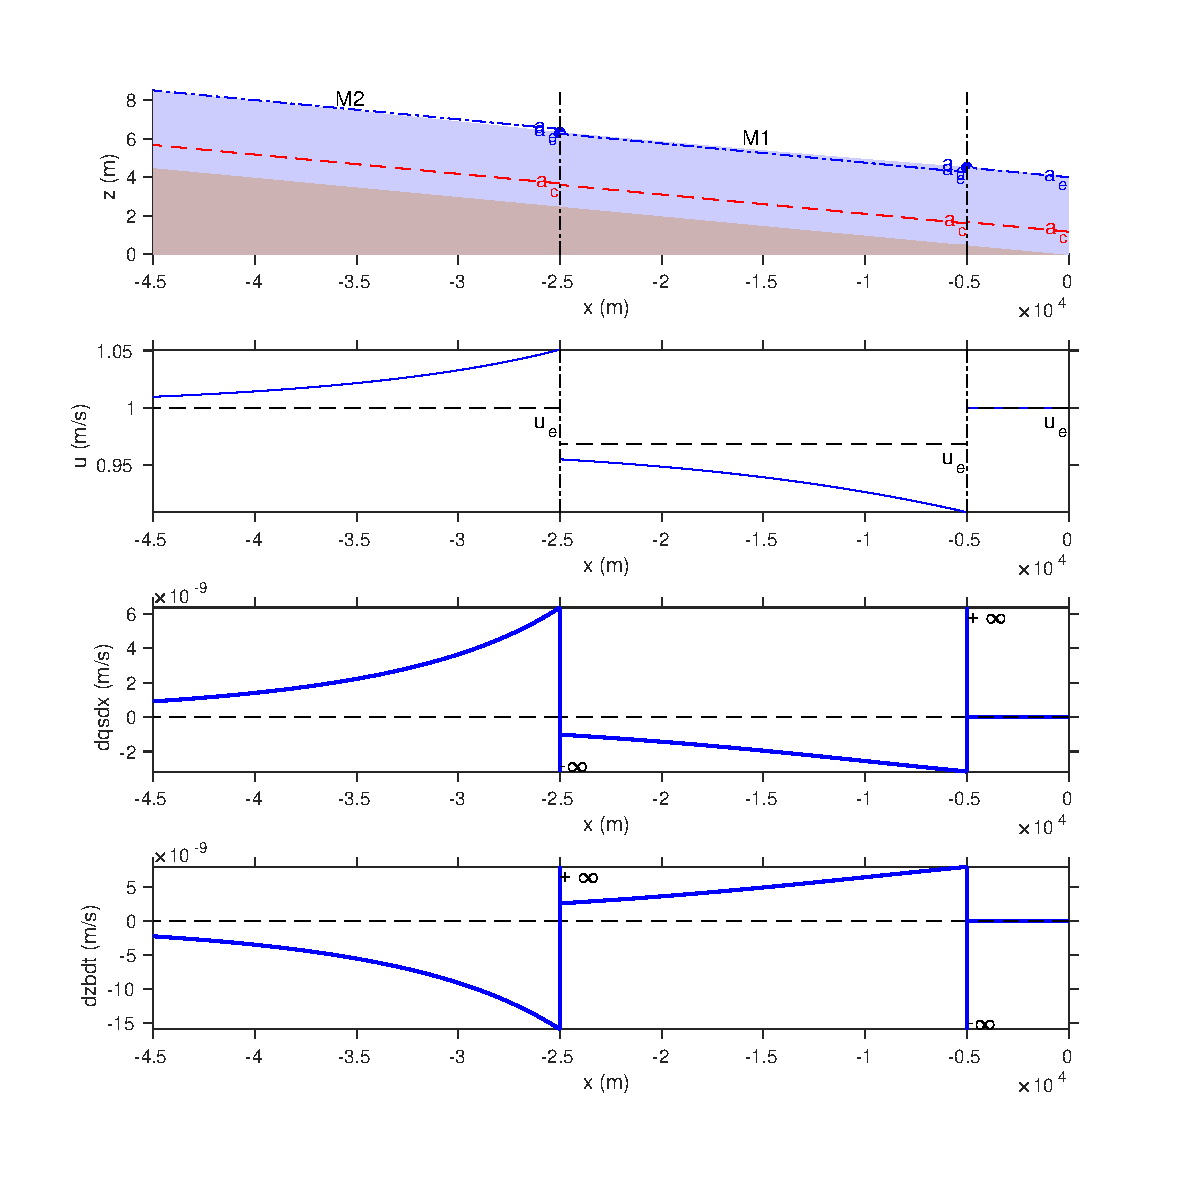
\includegraphics[width=\linewidth]{matlab/initersed_widening.pdf} 
  \caption{From backwater curve to initial erosion and sedimentation.}
  \label{fig:initersed_widening}
\end{figure}
\begin{exercise}
  Try to produce a figure similar to the middle panel in figure 12.2 of the lecture notes, by zooming into the figure you just produced.
\end{exercise}

\begin{solution}
  Plotting the backwater and zooming in on the transition you get something similar to \autoref{fig:zoom_backwater}.
  \begin{figure}
      \centering
  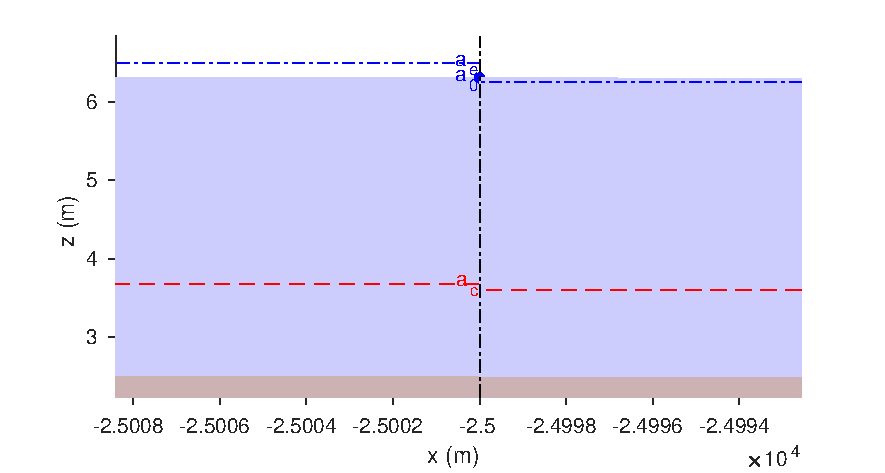
\includegraphics[width=\linewidth]{matlab/zoom_backwater.pdf}
      \caption{Zooming in on the transition at A we can create a figure similar to one in the lecture notes. Zooming in, the bed-slope is no longer visible.}
      \label{fig:zoom_backwater}
  \end{figure}

\end{solution}
\subsection{River bend cutoff}
\begin{exercise}
  Consider the case of a river bend cutoff discussed during the first pc practical. Make a figure of the initial erosion and sedimentation that you expect following the cutoff. Explain the graphs obtained.
\end{exercise}

\begin{solution}
After creating the cutoff backwaters in PC Practical 1, we can plot the initial erosion and sedimentation for the cutoff case:
\begin{lstlisting}
B.plot_initial_ersed
\end{lstlisting}
This results in a figure similar to \autoref{fig:cutoff_initersed}
\begin{figure}
    \centering
    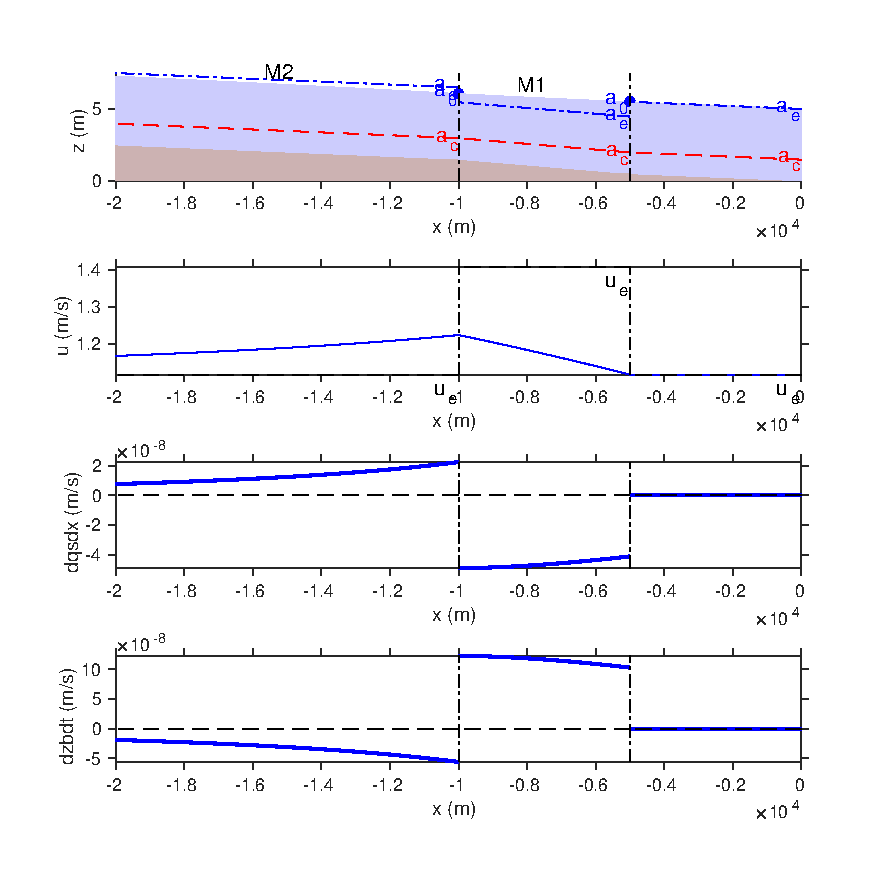
\includegraphics[width=\linewidth]{matlab/cutoff_initersed.pdf}
    \caption{Initial sedimentation and erosion after cutoff}
    \label{fig:cutoff_initersed}
\end{figure}
In the top panel of \autoref{fig:cutoff_initersed} the backwaters are reproduced. In the panel below we have a graph of the velocity. The dashed lines indicate the equilibrium velocity. The equilibrium velocity in the middle reach is larger due to the increased bed-slope. In the upstream reach the water depth drops in downstream direction and is below equilibrium depth. That explains why the velocity is larger than equilibrium velocity and increasing in downstream direction (continuity). In the middle reach velocity is lower than equilibrium depth and drops, due to the increasing depth. In the downstream reach velocity is at equilibrium.
The gradient in sediment transport follows the gradient in velocity. It is positive and increasing in the upstream part, than suddenly drops at the transition to the middle reach, becoming negative. This is because of the backwater, causing the flow to go from accelerating conditions to decelerating condition in the middle reach. In the downstream reach flow is uniform and the gradient in sediment transport is zero.
The rate of bed level change has opposite sign compared to the sediment transport gradient. The accelerating flow in the upstream part results in erosion. In the middle reach sedimentation occurs due to the decelerating flow loosing sediment to the bed. In the downstream part no erosion or sedimentation occurs.
\end{solution}

\section{Morphological equilibrium}
In this section we will evaluate the long term morphological development of a river (section 12.3 in the lecture notes).

\subsection{River widening}
The morphological equilibrium is determined by the influx of sediment into the river. Therefore we need to set the right sediment transport. For this we assume that the entire river was in morphological equilibrium before the widening. So we can compute the original sediment transport rate in equilibrium:
\begin{lstlisting}
[R.qs_morf_eq]=deal(R(1).m_sed_transp*R(1).u_equilibrium^R(1).n_sed_transp);
\end{lstlisting}
Here we used the simplified sediment transport formula. 
Now we can what the morphological equilibrium slopes and depths are for the widening case:
\begin{lstlisting}
>> [R.So_morf_equilibrium]

ans =

   1.0e-03 *

    0.1000    0.1100    0.1000

>> [R.a_morf_equilibrium]

ans =

    4.0000    3.6364    4.0000

>> 
\end{lstlisting}
You can see that for the widened reach the river will tend to develop a steeper slope and a smaller depth.
\begin{exercise}
  Explain why the river tends to develop a larger slope and a smaller depth in the widened section
\end{exercise}
\begin{solution}
In morphological equilibrium the river transports sediments at a constant rate along the river. This means that we need everywhere the same flow velocity. The river widening will be compensated by a drop in water level, which, to keep uniform conditions, requires a larger bed slope.
\end{solution}
We can produce a plot of the final morphological equilibrium by issuing:
\begin{lstlisting}
R.plot_morf_equilibrium()
\end{lstlisting}
This will produce \autoref{fig:morfeq_widening}
\begin{figure}[ht]
  \centering
  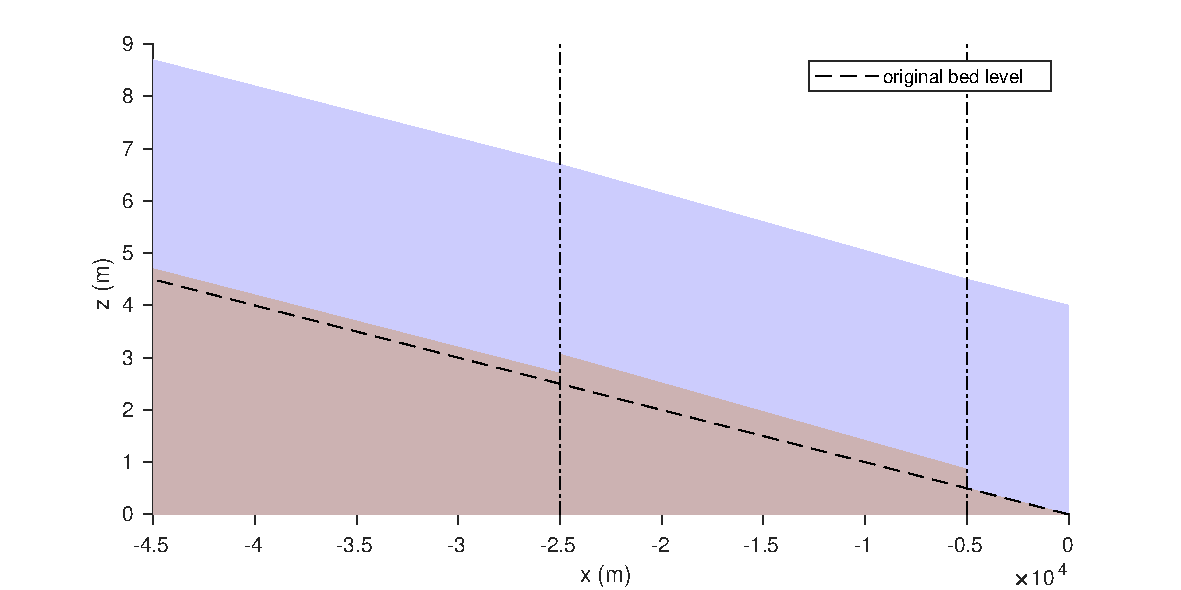
\includegraphics[width=\linewidth]{matlab/morfeq_widening.pdf}
  \caption{Morphological equilibrium at the widening}
  \label{fig:morfeq_widening}
\end{figure}

\subsection{River bend cutoff}

\begin{exercise}
  Determine the morphological equilibrium for the river cutoff and explain the new equilibrium that developed. What can you conclude regarding flood protection on the long run, after creating a river cutoff?
\end{exercise}
\begin{solution}
  Plotting the morphological equilibrium for the cutoff case we get \autoref{fig:cutoff_morf}. Overall the bed will erode upstream of the cutoff, while retaining the same equilibrium depth. This reduces flood risk.
\begin{figure}
    \centering
    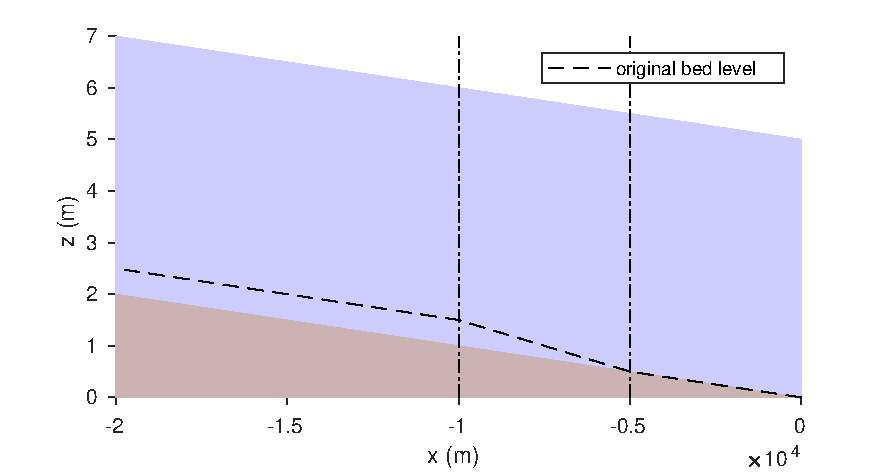
\includegraphics[width=\linewidth]{matlab/cutoff_morfeq.pdf}
    \caption{Morphological equilibrium for a river bend cutoff}
    \label{fig:cutoff_morfeq}
\end{figure}

\end{solution}

\section{Morphodynamics}
In this part you will use a solver of the hyperbolic equation for 1D morphodynamics found in section 12.6 of the lecture notes. For this part you will also need to download \lstinline{morf_solver.m} and \lstinline{plot_zb_sym.m} from brightspace.

We will start with a backwater object:
\begin{lstlisting}
B=Backwater;
\end{lstlisting}
For the morphodynamic computations we use the function \lstinline{morf_solver.m} that solves the hyperbolic 1D morphodynamic equation found in section 12.7 of the lecture notes.
This functions needs three inputs:
\begin{enumerate}
  \item A backwater object
  \item The initial condition for the bed
  \item The time at which the computation should end
\end{enumerate}
When called the function will return a matrix with the solved morphological development with the spatial coordinate defined in the first dimension and the temporal coordinate in the second dimension.
We will start with a simple example to show how it works. 
First we make a plot of the Backwater object we constructed:
\begin{lstlisting}
plot(B)
\end{lstlisting}
This produces \autoref{fig:backwater_morf}
\begin{figure}[ht]
  \centering
  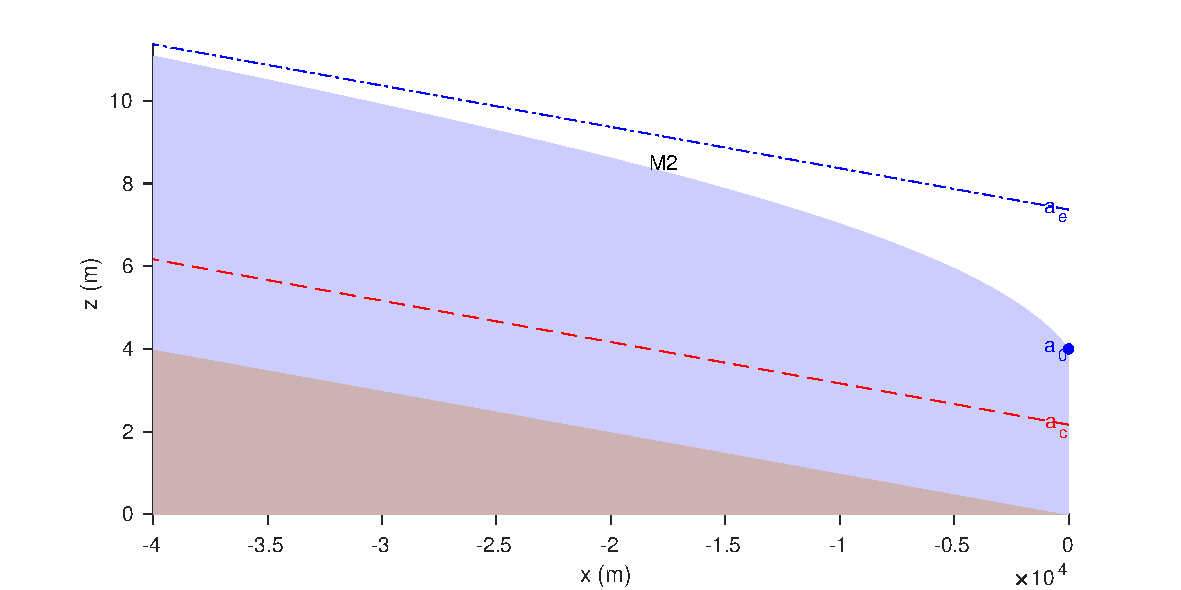
\includegraphics[width=\linewidth]{matlab/backwater_morf}
  \caption{Backwater case for the morphodynamic development}
  \label{fig:backwater_morf}
\end{figure}

For the morphodynamic computation we need to specify the initial condition as a deviation from the initial equilibrium bed. In this case we will try to simulate the morphodynamic development of dredged piece of river.
Let's say we dredge \SI{2}{\m} between $-\SI{20}{\kilo\m}<x<-\SI{15}{\kilo\m}$.
The bed changes need to be defined at the $x$ locations where the backwater is computed:
\begin{lstlisting}
x=B.x_curve; % get x where backwater is computed
delta_z=zeros(size(x)); % make a first vector to hold the bed changes
delta_z(x>-2e4 & x < -1.5e4)=-2;
\end{lstlisting}
You can plot \lstinline{x} vs \lstinline{delta_z} to check the result.
Now we can run the computation. Let's run the simulation for 3 months of development:
\begin{lstlisting}
[x, z_b_sym, dt]=morf_solver(B,delta_z,3*30*24*3600);
\end{lstlisting}
The function returns the $x$ locations where the solution is computed, the solved bed and the time step used in the computation.
\begin{exercise}
  Make a plot of the solution using the function \lstinline{imagesc}. In the figure you can see a diagonal line. What does this line represent?
\end{exercise}
We can animate the morphological development by using the \lstinline{plot_zb_sym.m} function. This takes as input the x-coordinate of the solution and the solution. Optionally you can specify the time step of the simulation, the duration of the produced animation and the bed slope of the river.
We will call it now with the first three arguments:
\begin{lstlisting}
plot_zb_sym(x,z_b_sym, dt) 
\end{lstlisting}
\begin{exercise}
  The behaviour you observe is obviously advective. Under which circumstances do you expect the morphodynamic behaviour to be advective?
\end{exercise}
Under some conditions the morphological development can be diffusive.
\begin{exercise}
  Modify the above case such that the morphodynamic behaviour becomes diffusive.
\end{exercise}

\printsolutions

\end{document}
